% Audit paper (second paper of the IPS project). First full draft, 2026-11-14.
% Numbers: docs/AUDIT_PAPER_PLAN.md sections 4.1-4.5 and results_cache/2026-11-0{9,10}, 2026-11-1{2,4}.
% Open items before submission (also in README.md next to this file):
%   TODO-1  read TOR-VIO (IJCNN'26) and Gu et al. (IEEE Sensors J. 2026); adjust the novelty claim of Sec. III.
%   TODO-2  compare the released UL-VIO and NASVIO checkpoints with the numbers printed in their papers.
%   TODO-3  confirm that RWKV-VIO, DB-VIO and DAP-Pose use the same imus/*.mat (Table I lists only checked repos).
%   TODO-4  verify the bibliography fields marked TODO in refs.bib.
%   TODO-5  contact the authors of VS-VIO, NASVIO, UL-VIO and VIFT before posting.
\documentclass[letterpaper,journal]{IEEEtran}
\usepackage{amsmath,amssymb}
\renewcommand{\ttdefault}{cmtt}  % Courier (pcr) is not installed here
\usepackage{graphicx}
\usepackage{booktabs}
\usepackage{array}
\usepackage{xcolor}
\usepackage{url}
\usepackage{cite}
\usepackage[hidelinks]{hyperref}

\newcommand{\trel}{t_{\mathrm{rel}}}
\newcommand{\rrel}{r_{\mathrm{rel}}}
\newcommand{\todo}[1]{\textcolor{red}{[TODO: #1]}}

\begin{document}

\title{What the KITTI Benchmark Measures in Learned\\Visual--Inertial Odometry: A Timing Error,\\Test-Set Selection, and Seed Variance}

\author{Nada El Madah%
\thanks{Draft, 2026-11-14. Code, Kaggle kernels, corrected inertial files and every score in this paper: to be released.}}

\markboth{Preprint, 2026}{What the KITTI Benchmark Measures in Learned VIO}

\maketitle

\begin{abstract}
Learned visual--inertial odometry (VIO) methods are ranked by their translation error $\trel$ on KITTI sequences 05, 07 and 10, and published gaps between methods are often a few tenths of a percent. We audit what this number measures. (i)~\emph{Data.} The inertial files used by VS-VIO, NASVIO, UL-VIO and VIFT are byte-identical; they store 11 samples per image pair, which suggests 10\,ms steps, but the samples span the true image interval of $\approx$104\,ms and lag the images by $\approx$60\,ms. Integrating them with the nominal step under-rotates every frame by 4\% (gyroscope-only rotation: 4.62\% $\trel$ instead of 1.70\%). Correcting the lag before training does not change the network measurably (six paired seeds, $p=0.57$). (ii)~\emph{Protocol.} In every released training script we checked, sequence 08 is in the training set and the checkpoint is chosen on 05/07/10, the test sequences. (iii)~\emph{Variance.} Retraining VIFT with six seeds under one protocol spans 2.38--4.04\%, wider than the 2.35--3.88\% spread of five released configurations of three methods; retraining VS-VIO end to end spans 3.55--6.83\%, and choosing its epoch on the test sequences lowers the reported number by 0.89 on average. Under a clean protocol (08 held out, no test-set selection), VS-VIO's own code gives 3.55--6.83\% against 2.35\% for its released checkpoint, with a one-GPU control at the authors' default setting confirming the gap. (iv)~\emph{Diagnosis.} Replacing pose components with ground truth or with sensor measurements shows that rotation is the largest error source of every released model; once rotation comes from the gyroscope and step length from the accelerometer, seed spread falls to 0.07 while the spread between methods stays at 0.47, so only then does a ranking carry information. We release corrected inertial files, a clean protocol and scripts that re-score any model under it.
\end{abstract}

\begin{IEEEkeywords}
Visual--inertial SLAM, deep learning methods, performance evaluation and benchmarking, sensor fusion.
\end{IEEEkeywords}

\section{Introduction}

\IEEEPARstart{L}{earned} VIO regresses the relative pose between two camera frames from images and inertial measurements with a neural network \cite{Clark2017,Han2019,Yang2022,Kurt2024}. Since VS-VIO \cite{Yang2022}, most methods are compared on the KITTI odometry benchmark \cite{Geiger2012,Geiger2013} with the same data pipeline: training on sequences 00--09 except 03, 05 and 07, testing on 05, 07 and 10, and reporting the mean relative translation error $\trel$ and rotation error $\rrel$ of the test sequences. Reported numbers have fallen from 2.35\% for the released VS-VIO checkpoint to 1.96\% for VIFT \cite{Kurt2024} and 1.69--1.77\% for later work \cite{Ma2026,Wan2026}, so successive improvements are a few tenths of a percent.

Whether such differences reflect better models depends on three things that published tables do not show: whether the inputs are what the methods assume, whether the test sequences influence training, and how much a single method varies with its random seed. We audit all three on four methods whose code is public and on retrained models, and add a component-wise diagnosis that says which part of the pose each model gets wrong.

\textbf{Contributions.}
\begin{enumerate}
\item \emph{A timing error in shared inertial data} (Sec.~\ref{sec:data}). The KITTI inertial files used across learned-VIO repositories assume 10\,ms steps that are in fact $\approx$10.4\,ms, and lag the images by $\approx$60\,ms. We measure the effect on gyroscope integration and on a network retrained with corrected files.
\item \emph{A protocol audit} (Sec.~\ref{sec:protocol}) of the released training code: sequence 08 is trained on and checkpoints are selected on the test sequences.
\item \emph{A variance study} (Sec.~\ref{sec:variance}): seed spread of two methods retrained from their own code, the effect of best-of-$k$ seed selection and of test-set epoch selection, and a clean-protocol retraining of VS-VIO with two controls.
\item \emph{A component-wise diagnosis} (Sec.~\ref{sec:diag}) of the released models of three methods by oracle swap and sensor substitution, showing what remains different between methods once measurable components are measured.
\item Corrected inertial files, a clean protocol and re-scoring scripts (Sec.~\ref{sec:recs}).
\end{enumerate}
Every number in this paper comes from public code and data and from Kaggle kernels that we release; none of the audited models was trained by us unless we say so.

\section{Benchmark and Evaluation}
\label{sec:bench}

\textbf{Data.} KITTI odometry provides stereo images at $\approx$10\,Hz and ground-truth poses for sequences 00--10 \cite{Geiger2012}. Inertial data come from the raw recordings (OXTS RT3003, 100\,Hz) \cite{Geiger2013}; VS-VIO distributes them as one \texttt{imus/<seq>.mat} file per sequence, with 11 samples for each image pair, and later methods load these files unchanged (Table~\ref{tab:repos}). Models see non-overlapping windows of 11 frames; recurrent models carry their state across windows at test time.

\textbf{Metrics.} $\trel$ (\%) and $\rrel$ (deg/100\,m) follow the KITTI odometry protocol, averaged over subsequences of 100--800\,m and over the three test sequences. All scores in this paper use one implementation, checked against the authors' evaluation on the released VS-VIO checkpoint (2.04/1.64/3.38\% on 05/07/10, matching the 2.04/1.64/3.35\% reported in the VS-VIO repository).

\textbf{An independent reference.} KITTI ground truth for these sequences is computed from the same OXTS unit that supplies the inertial data. Every main result is therefore repeated against SuMa lidar poses \cite{Behley2018}, which do not use the IMU; SuMa numbers are $\approx$0.1 higher throughout and never change a conclusion.

\textbf{Pose components.} We write a relative pose as rotation, translation direction and step length. An \emph{oracle swap} replaces one component of the prediction by ground truth and re-scores \cite{Cimarelli2022}; a \emph{sensor substitution} replaces it by a measurement: rotation integrated from the gyroscope over the true image interval and lag, step length from the accelerometer, and finally the frozen observability gate of \cite{ElMadah2026gate}, which chooses per frame pair between the network and the measurements from sensor signals alone. The gate was fixed on held-out data before any model in this paper was scored, and is applied unchanged.

\section{The Inertial Data}
\label{sec:data}

\begin{table}[t]
\centering
\caption{Released learned-VIO code on KITTI. ``Same .mat'': \texttt{imus/05.mat} byte-identical (MD5) to VS-VIO's. Training sets and validation sets as in the released training scripts.}
\label{tab:repos}
\setlength{\tabcolsep}{3pt}
\begin{tabular}{@{}lcccc@{}}
\toprule
Method & Same .mat & 08 in training & Validation set & Weights \\
\midrule
VS-VIO \cite{Yang2022} & reference & yes & 05/07/10 & yes \\
NASVIO \cite{Chen2023NASVIO} & yes & yes & 05/07/10 & yes \\
UL-VIO \cite{Park2024ULVIO} & yes & ---$^a$ & ---$^a$ & yes \\
VIFT \cite{Kurt2024} & yes & yes & 05/07/10$^b$ & no \\
\bottomrule
\multicolumn{5}{@{}p{0.95\columnwidth}@{}}{\footnotesize $^a$evaluation code only. $^b$the same split serves as validation and test; checkpointing and early stopping monitor its loss.}
\end{tabular}
\end{table}

\textbf{What the files contain.} Comparing the files with the raw OXTS recordings shows that each window of 11 samples is the 100\,Hz signal interpolated at 10 equal steps over the \emph{actual} interval between the two images (RMSE $\le 3.5\times10^{-4}$\,rad/s against the raw signal). That interval is 103.7--104.1\,ms on sequences 04--10, not 100\,ms. Fitting the offset that best aligns integrated gyroscope rotation with ground truth gives a lag of $+60$\,ms between inertial samples and images ($+65$\,ms against SuMa); we estimate it on training sequences only. The raw OXTS data also have gaps (1.62\,s in 05, 1.74\,s at the start of 06) that the files bridge by interpolation. Fig.~\ref{fig:timing} draws one frame pair to scale.

\begin{figure}[t]
\centering
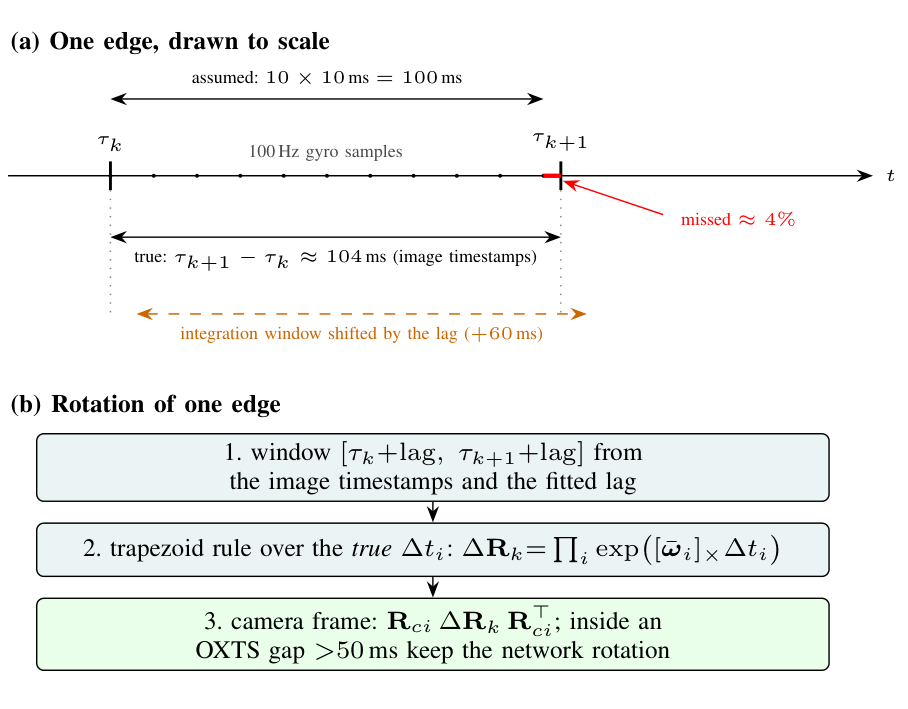
\includegraphics[width=\columnwidth]{figures/gyro_timing.png}
\caption{One KITTI frame pair to scale. The inertial files imply $10\times10$\,ms; the images are $\approx$104\,ms apart, and the inertial samples lag them by $\approx$60\,ms. (b)~Rotation over the true interval and lag, as used for gyroscope substitution.}
\label{fig:timing}
\end{figure}

\textbf{Effect on integration.} A method that integrates these samples with the nominal 10\,ms step under-rotates every frame by $\approx$4\%, which makes an accurate gyroscope look biased. With VIFT's translation, gyroscope rotation integrated with the nominal step gives 4.62\% $\trel$, worse than the network; integrated over the true interval and lag it gives 1.70\%, with per-frame rotation errors of 0.023--0.037$^\circ$ and $\rrel$ 0.18. Any physics-informed, hybrid or filter-based method built on these files inherits the error unless it reconstructs the timing. To our knowledge this has not been reported: a VS-VIO issue asks why each pair has 11 samples without reaching the timing, and later work describes KITTI as hardware-synchronized \cite{DAPPose}. \todo{confirm against TOR-VIO \cite{TORVIO2026} and Gu et al.\ \cite{Gu2026} before claiming priority.}

\textbf{Effect on a network.} A network does not see the step size, but it does see the lag. We rebuilt the files with VS-VIO's own interpolation evaluated at image time plus lag (with zero lag the script reproduces the released files to $4\times10^{-4}$\,rad/s, the rounding level of OXTS) and retrained VIFT's transformer on them, six seeds paired with six baselines that differ only in the files (Table~\ref{tab:e4}). The network number does not move: 2.79$\pm$0.62 against 2.56$\pm$0.42, better in 3 of 6 pairs ($p=0.57$, paired $t$; $p=1.00$, Wilcoxon). The translation of the network may improve slightly ($-0.10$ with ground-truth rotation, $p=0.06$), and after sensor substitution the difference is $-0.04$ ($p\approx0.2$). The timing error is therefore a data defect that harms integration-based methods; it does not decide the accuracy of networks trained on the same files. The VIFT encoder stays frozen in this experiment and was trained on the lagged files, so a network trained end to end on corrected data may behave differently.

\begin{table}[t]
\centering
\caption{Lag-corrected inertial files, VIFT retrained under the clean protocol, six paired seeds. $\trel$ (\%), 05/07/10, OXTS.}
\label{tab:e4}
\setlength{\tabcolsep}{1.8pt}
\begin{tabular}{@{}lcccc@{}}
\toprule
Stage & Released files & Lag-corrected & Mean diff. & $p$ ($t$ / W) \\
\midrule
Network & 2.79$\pm$0.62 & 2.56$\pm$0.42 & $-0.23$ & 0.57 / 1.00 \\
GT rot.\ + net transl. & 1.99$\pm$0.05 & 1.90$\pm$0.09 & $-0.10$ & 0.06 / 0.13 \\
Gyro rot.\ + net transl. & 2.13$\pm$0.04 & 2.04$\pm$0.09 & $-0.09$ & 0.08 / 0.16 \\
+ accel.\ length & 1.64$\pm$0.03 & 1.61$\pm$0.06 & $-0.04$ & 0.25 / 0.19 \\
Gate \cite{ElMadah2026gate} & 1.58$\pm$0.03 & 1.53$\pm$0.06 & $-0.04$ & 0.22 / 0.16 \\
Gate vs.\ SuMa & 1.67$\pm$0.04 & 1.62$\pm$0.06 & $-0.04$ & 0.21 / 0.16 \\
\bottomrule
\end{tabular}
\end{table}

\section{The Protocol}
\label{sec:protocol}

The published papers describe a training set without the test sequences, but the released code goes further (Table~\ref{tab:repos}). VS-VIO's \texttt{train.py} trains on 00, 01, 02, 04, 06, 08 and 09, evaluates on 05, 07 and 10 after every epoch of the last stage, and saves the checkpoint with the lowest test $\trel$. VIFT's latent-caching script trains on the same seven sequences and uses 05/07/10 as validation and test at once; its checkpointing and early stopping monitor the loss on these sequences. NASVIO trains on 08 and validates on 05/07/10 each epoch. RWKV-VIO's code keeps the best test $\trel$ while its paper reports the last epoch \cite{RWKVVIO2025}; DeepVIO trains on 00--08, which contains 05 and 07 \cite{Han2019}, so its numbers are not comparable with the 05/07/10 column of later tables.

Two effects follow. Sequence 08 adds about 25\% of the training windows; in our VIFT reproduction, training with 08 under the released code gives 2.11\% and the split described in the paper 2.54--2.55\%. Selecting on the test sequences adds an optimistic bias whose size we measure in Sec.~\ref{sec:variance}. Reproducibility suffers in smaller ways too: NASVIO's test script reads ground-truth files that the released code does not build (the preprocessing script stops at a debugger breakpoint), and we rebuilt them with the authors' own function.

\section{How Large Are the Differences?}
\label{sec:variance}

\textbf{Seed spread of a frozen-encoder model.} Seed variance is a known hazard of deep-learning benchmarks \cite{Henderson2018,Bouthillier2021,Musgrave2020}; we measure it here. We retrained VIFT six times under the clean protocol (training without 08, checkpoint chosen on 08), with the same code and data and only the seed changed. The network $\trel$ spans 2.38--4.04\% (SD 0.62). The four released checkpoints of three methods, scored as five configurations (VS-VIO with its learned visual selection and with vision always on), span 2.35--3.88\% (Fig.~\ref{fig:spread}, Table~\ref{tab:spread}): every released model falls inside the seed range of a single method. Keeping the best of $k$ seeds by test score, as a paper that selects on the test sequences implicitly does, lowers the expected network number from 2.79 ($k=1$) to 2.50, 2.46 and 2.38 for $k=2,3,6$.

\begin{figure}[t]
\centering
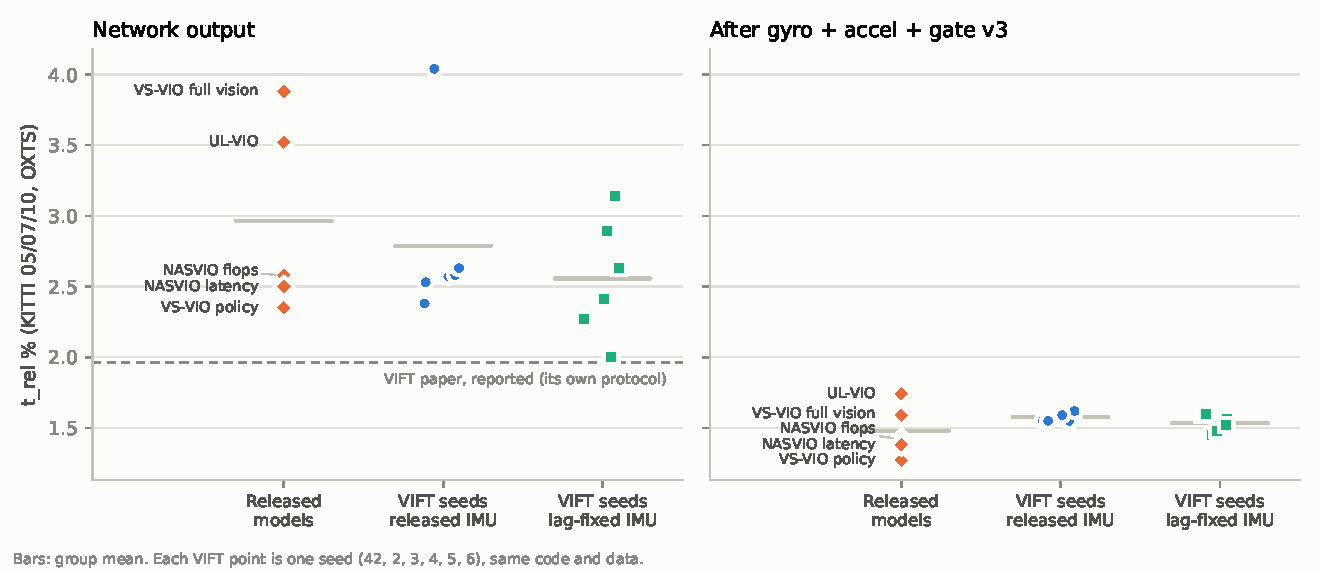
\includegraphics[width=\columnwidth]{figures/audit_e6_spread.pdf}
\caption{Five released configurations of three methods against six seeds of one method (VIFT, released and lag-corrected inertial files). Left: network output. Right: after gyroscope rotation, accelerometer step length and the frozen gate.}
\label{fig:spread}
\end{figure}

\begin{table}[t]
\centering
\caption{Spread between methods and between seeds, $\trel$ (\%), 05/07/10, OXTS: min--max (range).}
\label{tab:spread}
\setlength{\tabcolsep}{1.5pt}
\begin{tabular}{@{}lccc@{}}
\toprule
Stage & 5 released & VIFT, 6 seeds & VS-VIO, 3 seeds$^a$ \\
\midrule
Network & 2.35--3.88 (1.53) & 2.38--4.04 (1.66) & 3.55--6.83 (3.28) \\
Gyro rot.\ + net transl. & 1.71--2.17 (0.46) & 2.06--2.18 (0.12) & 3.49--4.00 (0.51) \\
+ accel.\ length & 1.38--1.82 (0.44) & 1.61--1.69 (0.08) & 2.66--3.05 (0.39) \\
Gate \cite{ElMadah2026gate} & 1.27--1.74 (0.47) & 1.55--1.62 (0.07) & 2.56--2.98 (0.42) \\
\bottomrule
\multicolumn{4}{@{}p{0.95\columnwidth}@{}}{\footnotesize $^a$retrained end to end, epoch chosen on 08 (Sec.~\ref{sec:e5}).}
\end{tabular}
\end{table}

\textbf{Seed spread of an end-to-end model.} VIFT trains a transformer on a frozen encoder, which may understate the variance of models trained from scratch. We therefore retrained VS-VIO from its released code (commit \texttt{27b06b3}) under the clean protocol with seeds 0, 1 and 2, 100 epochs each, and recorded every epoch the authors evaluate (81--99). With the epoch chosen on 08 the network spans 3.55--6.83\% (SD 1.67), about twice the spread of VIFT.

\textbf{Test-set epoch selection.} Within one run, the test error of VS-VIO jumps between consecutive epochs of the fine-tuning stage (seed 0: 3.50--7.14\%) although the learning rate is $10^{-6}$. These jumps are real changes of the model, not evaluation noise: re-evaluating one checkpoint with three seeds of the stochastic visual-selection policy varies by 0.03--0.22. Choosing the epoch with the lowest test error, the rule in VS-VIO's \texttt{train.py}, gives a number 0.86, 0.97 and 0.83 below the median epoch of the three seeds (mean 0.89). Choosing on 08 gains less, because 08 tracks the test error across epochs in two seeds (Spearman $+0.93$) but not in the third ($-0.49$). Fig.~\ref{fig:e5} shows the epoch curves and the three selection rules.

\textbf{After sensor substitution.} With gyroscope rotation, accelerometer length and the gate, the picture changes (Table~\ref{tab:spread}). VIFT's seed spread falls from 1.66 to 0.07 (SD 0.03), while the spread between the released methods stays at 0.47, seven times larger; VS-VIO policy and both NASVIO checkpoints are better than all twelve VIFT runs, and UL-VIO is worse. Best-of-$k$ selection now changes almost nothing (1.58 to 1.55 for $k=6$), and neither does test-set epoch selection for VS-VIO ($-0.01$ on average). Most of the variance of the network number lies in components that the sensors measure.

\section{Retraining VS-VIO Under a Clean Protocol}
\label{sec:e5}

\begin{table}[t]
\centering
\caption{VS-VIO retrained from its released code, 08 held out. $\trel$ (\%), 05/07/10, OXTS; mean$\pm$SD over seeds 0/1/2 (two GPUs); one-GPU control: seed 0 at the authors' default.}
\label{tab:e5}
\setlength{\tabcolsep}{2.5pt}
\begin{tabular}{@{}lcccc@{}}
\toprule
Epoch rule & Network & Gyro + net & + accel. & Gate \\
\midrule
Best on 08 (clean) & 5.02$\pm$1.67 & 3.81$\pm$0.28 & 2.88$\pm$0.20 & 2.80$\pm$0.22 \\
Best on test (authors') & 4.69$\pm$1.19 & 3.79$\pm$0.13 & 2.88$\pm$0.07 & 2.79$\pm$0.07 \\
Last epoch & 6.48$\pm$1.46 & 3.79$\pm$0.14 & 2.92$\pm$0.05 & 2.83$\pm$0.07 \\
\midrule
One GPU, best on 08 & 4.53 & 3.78 & 2.66 & 2.61 \\
One GPU, best on test & 3.80 & 3.65 & 2.60 & 2.54 \\
\midrule
Released checkpoint & 2.35 & 1.81 & 1.38 & 1.27 \\
\bottomrule
\end{tabular}
\end{table}

\begin{figure*}[t]
\centering
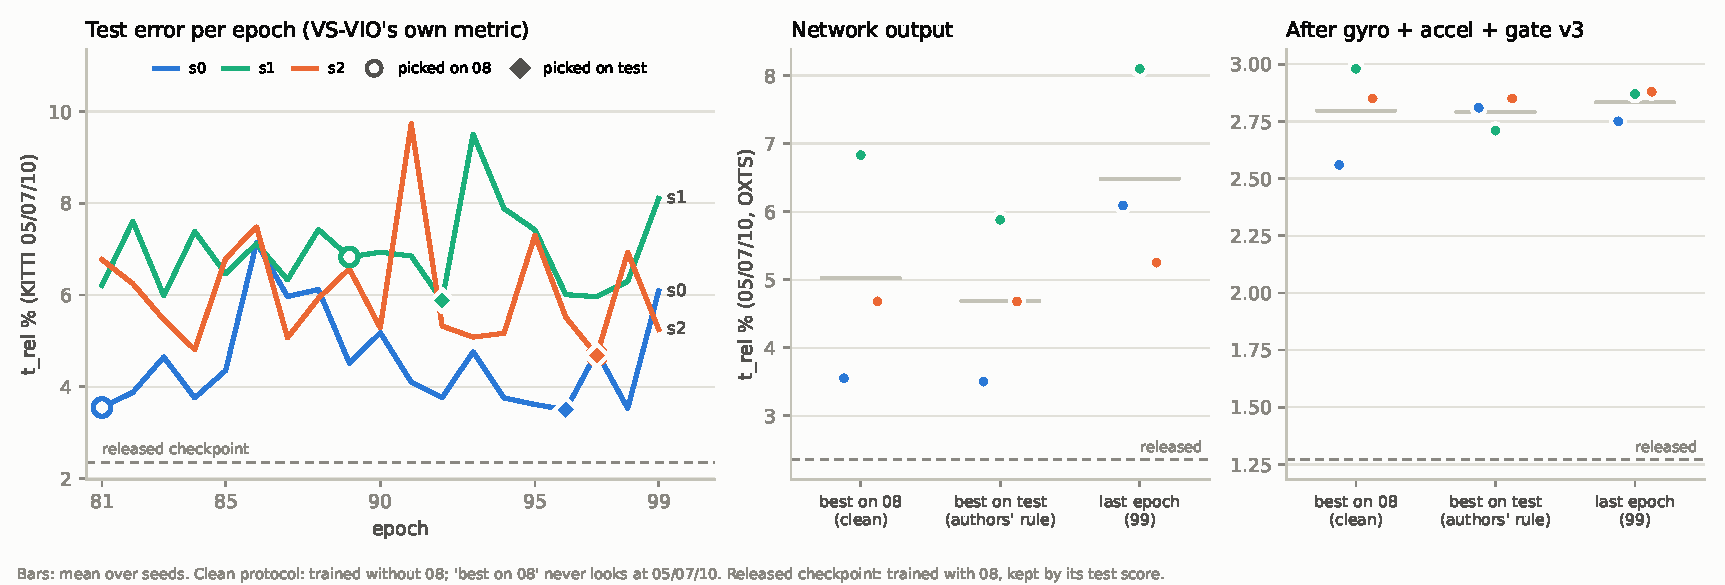
\includegraphics[width=0.92\textwidth]{figures/audit_e5.pdf}
\caption{VS-VIO retrained under the clean protocol, seeds 0--2. Left: test error of every evaluated epoch (VS-VIO's own metric), with the epoch picked on 08 (circle) and on the test sequences (diamond). Middle and right: the three epoch rules for the network and after sensor substitution; dashed line: released checkpoint.}
\label{fig:e5}
\end{figure*}

Table~\ref{tab:e5} lists the retrained VS-VIO under three epoch rules. All runs are far worse than the released checkpoint: the network gives 3.5--6.8\% against 2.35\%, and after sensor substitution 2.5--3.0\% against 1.27\%. On the same frames, rotation is as accurate as the released model (per-axis correlation with ground truth 0.99 in both), but the retrained models overestimate forward motion by 4--8\% where the released one does so by 1.5--2.5\%. The gap persists after accelerometer step length (2.66--3.05\% against 1.38\%), so it is not only a matter of scale.

Because the gap is large, we ruled out our own setup with two controls. Our runs split each batch of 16 across two GPUs, while the authors' default is one GPU, so batch-normalisation statistics were estimated from 8 samples. \emph{(a)~Statistics.} Re-estimating every batch-normalisation statistic on the clean training split with batches of 16, without changing a weight, moves the saved statistics by at most 0.02 standard deviations in the image and inertial encoders, makes all four models worse (the released one as well, 1.32 to 1.55 after the gate) and leaves the scale overestimate in place (1.06--1.08 against 1.02). \emph{(b)~Training.} Retraining seed 0 on one GPU, the authors' default and otherwise identical (same initialisation and batch order), gives a median test error over epochs 81--99 of 4.29\% against 4.36\% on two GPUs, 2.61\% against 2.56\% after the gate, the same scale overestimate, and mean training losses within 3\% in each of the three training stages.

With VS-VIO's released code at its default setting, holding out 08 and not selecting on the test sequences therefore gives a network $\trel$ of 3.5--6.8\%, not 2.35\%. We cannot attribute the whole gap to removing 08: the released checkpoint may also come from a training run that differs from the released code (library versions, or selection among several runs on the test score), which we cannot reproduce. We report the number as what the released code produces under a clean protocol.

\section{What Each Model Gets Wrong}
\label{sec:diag}

\begin{table}[t]
\centering
\caption{Released checkpoints of three methods (all trained with 08); VS-VIO is one checkpoint run with its learned visual selection and with vision always on. $\trel$ (\%), 05/07/10, OXTS ($\rrel$ in parentheses); last column against SuMa.}
\label{tab:diag}
\setlength{\tabcolsep}{2pt}
\begin{tabular}{@{}lcccccc@{}}
\toprule
Model & Network & GT rot. & Gyro rot. & + accel. & Gate & Gate$_\mathrm{SuMa}$ \\
\midrule
VS-VIO policy & 2.35 (0.88) & 1.68 & 1.81 (0.17) & 1.38 & \textbf{1.27} & 1.30 \\
VS-VIO full vis. & 3.88 (1.57) & 2.01 & 2.12 (0.17) & 1.69 & \textbf{1.59} & 1.68 \\
UL-VIO & 3.52 (1.73) & 2.03 & 2.17 (0.18) & 1.82 & \textbf{1.74} & 1.84 \\
NASVIO flops & 2.58 (0.70) & 1.64 & 1.79 (0.18) & 1.47 & \textbf{1.42} & 1.54 \\
NASVIO latency & 2.50 (0.69) & 1.56 & 1.71 (0.18) & 1.43 & \textbf{1.38} & 1.50 \\
\bottomrule
\end{tabular}
\end{table}

Table~\ref{tab:diag} applies the oracle swap and the sensor substitution to the four released checkpoints (five configurations). The pattern is the same for all three methods. Rotation is the largest error source: ground-truth rotation with the network's own translation lowers $\trel$ by 28--48\%. Gyroscope rotation over the true interval comes close to this oracle ($\rrel$ 0.17--0.18 for every model against 0.69--1.73 for the networks), accelerometer step length lowers the error further, and the frozen gate lowers it by 45--59\% in total, on models we did not train and without changing a parameter. The ranking NASVIO latency $<$ NASVIO flops $<$ UL-VIO survives, but the gap shrinks from 1.0 to 0.4: a large part of the published difference lies in rotation, which a gyroscope measures, rather than in what the networks learned.

Two checks on the released checkpoints. On 08, which every released model was trained on, NASVIO gives 1.37--1.53\%, clearly below its test error as expected for training data, whereas UL-VIO gives 3.36\%, close to its test error of 3.52\%. \todo{compare with the numbers printed in the UL-VIO and NASVIO papers \cite{Park2024ULVIO,Chen2023NASVIO}; the released UL-VIO weights may differ from the paper's model or omit its test-time adaptation, which we did not run.}

\section{Recommendations}
\label{sec:recs}

\begin{enumerate}
\item \emph{Split.} Train on 00, 01, 02, 04, 06, 09, select on 08, test on 05, 07, 10, and never evaluate the test sequences during training. Report the selection rule; the last epoch is an acceptable alternative.
\item \emph{Seeds.} Report the mean and SD of at least three seeds. On this benchmark a single-seed difference below $\approx$1\% in network $\trel$ is within the seed spread of one method.
\item \emph{Inertial timing.} Use the true image interval and the $+60$\,ms lag when integrating; we release corrected files and the script that builds them from raw OXTS, which reproduces the original files at zero lag.
\item \emph{Diagnostics.} Report the oracle-swap and sensor-substitution rows next to the network number. They show where a model's error lies and remove most of the seed variance, so differences between methods become measurable.
\item \emph{References.} Report $\trel$ against SuMa as well as OXTS ground truth, since the latter shares its sensor with the inertial input.
\item \emph{Release.} Release weights, the exact training command and the code that builds every file the evaluation reads.
\end{enumerate}

\section{Limitations}

Seed variance is measured on two methods (six VIFT seeds, three plus one VS-VIO seeds); other architectures may vary more or less. The lag-corrected retraining keeps VIFT's frozen encoder, which was trained on the lagged files. The clean-protocol gap of VS-VIO cannot be split between removing 08 and differences between the released code and the authors' training run. The sensor substitution relies on OXTS inertial data, which also produce the ground truth; SuMa results agree throughout, but SuMa has its own drift. Finally, we audited four methods with public code; methods without code could not be checked.

\section{Conclusion}

On KITTI 05/07/10, the $\trel$ of a learned VIO network mixes a timing defect in shared inertial files, a protocol that lets the test sequences choose the checkpoint, and a seed variance larger than the published differences between methods. None of these is visible in a results table. Measured components remove most of the variance and leave differences between methods that are real; we recommend reporting them, together with a held-out 08, several seeds and the released code, so that the next improvement of a few tenths can be told apart from the next lucky seed.

\bibliographystyle{IEEEtran}
\bibliography{refs}

\end{document}
